\question{Câu 9}

Cho mạch khuếch đại tín hiệu như hình vẽ. Mạch có $V_{CC}=9\,\textsf{V}$. BJT $Q_{1}$ và $Q_{2}$ có hệ số $\beta = 100$. Các hệ số $V_{A} = \infty$.

\begin{figure}[H]
	\centering
	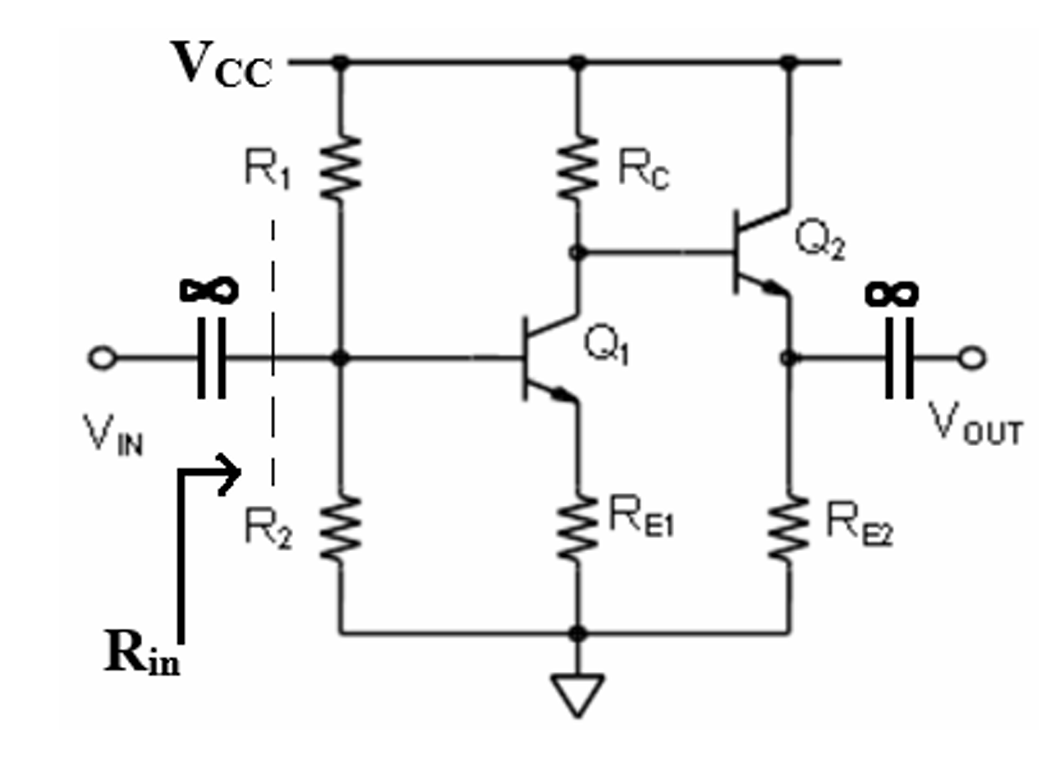
\includegraphics[width=.7\linewidth]{./my-chapters/my-images/Question9/debai.png}
\end{figure}

\answer{a}{Thiết kế mạch để có $Q_{1}(0.5\textsf{mA,} 3\,\textsf{V})$; $Q_{2}(2\,\textsf{mA,} 6\,\textsf{V})$.}

Sweep bf cho đến khi thỏa mãn điểm $Q$
	
	\begin{figure}[H]
		\centering
		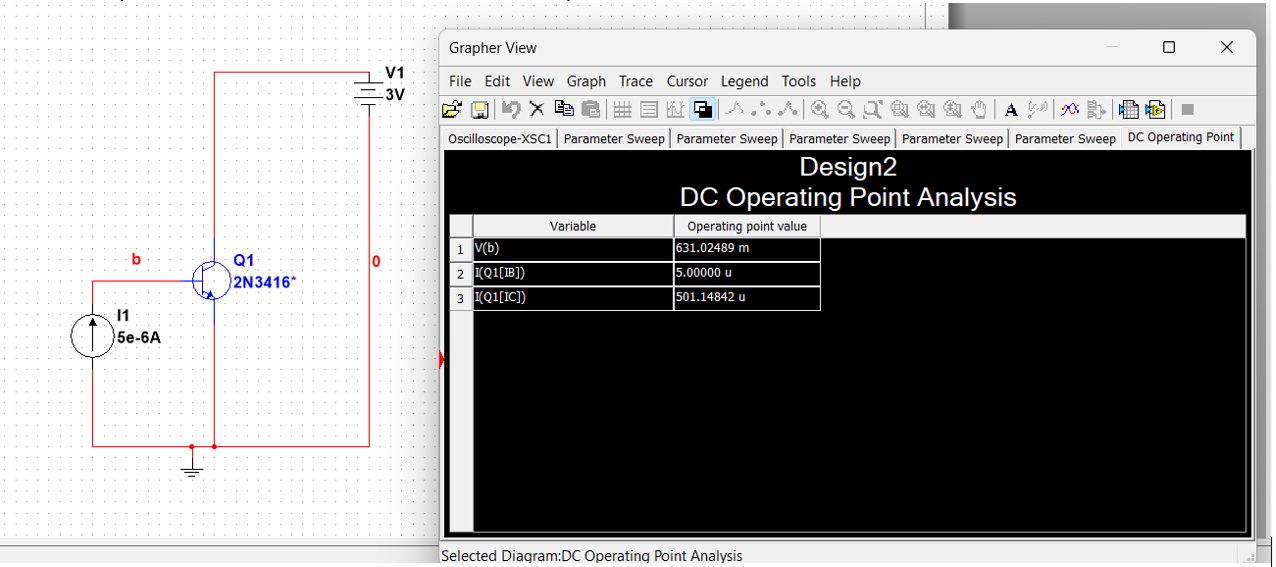
\includegraphics[width=.8\linewidth]{./my-chapters/my-images/Question9/a_sweep_timq.png}
		\caption{Chọn trasistor $Q_{1}$ thỏa mãn $\beta = 100$ ứng với $I_{C1} = 0.5 \,\textsf{mA}$ và $V_{CE1} = 3\,\textsf{V}$( chọn NPN 2N3416 với thông số bf chỉnh thấp còn $153$ so với $157$ ban đầu ); $V_{be} = 0.63 \,\textsf{V}$}
	\end{figure}
	
	\begin{figure}[H]
		\centering
		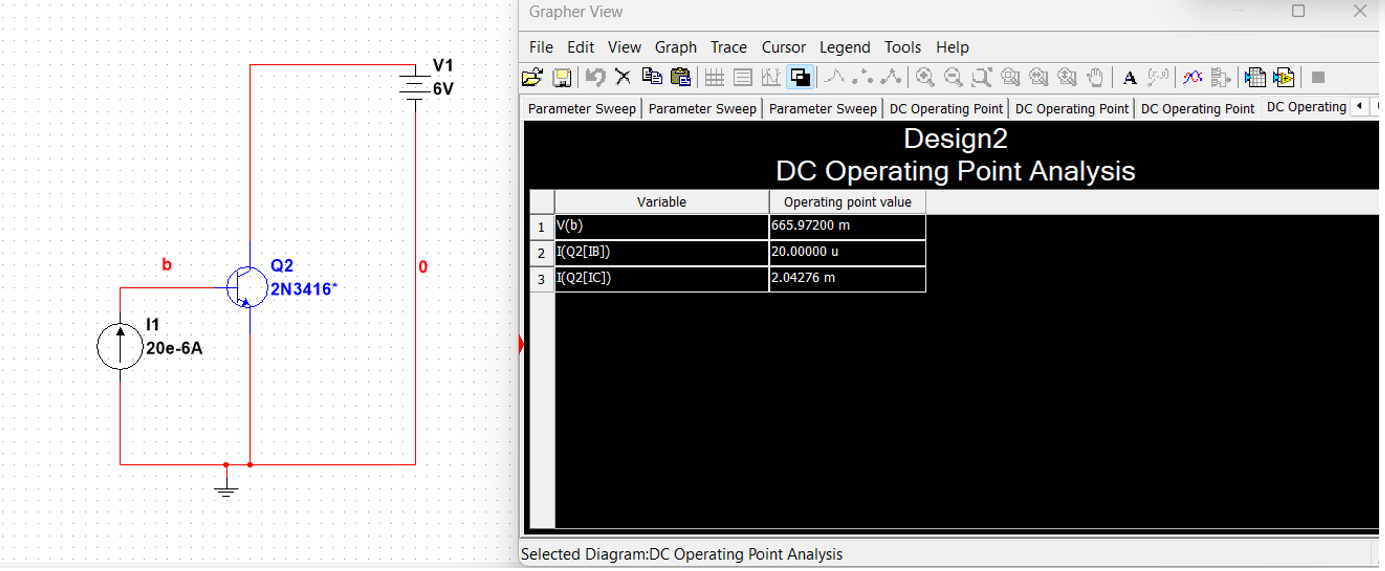
\includegraphics[width=.8\linewidth]{./my-chapters/my-images/Question9/a_sweep_timq_2.png}
		\caption{Chọn trasistor $Q_{2}$ thỏa mãn $\beta = 100$ ứng với $I_{C2} = 2 \,\textsf{mA}$ và $V_{CE2} = 6\,\textsf{V}$( chọn NPN 2N3416 với thông số bf chỉnh thấp còn $112$ so với $157$ ban đầu ); $V_{be} = 0.665 \,\textsf{V}$}
	\end{figure}
	
	\[
	R_{TH} = R_1 // R_2 \tag{1}
	\]
	
	\[
	V_{TH} = \frac{R_2}{R_1 + R_2} \, V_{CC} \tag{2}
	\]
	
	\[
	V_{TH} - V_{BE1} = I_{C1} \left( \frac{R_{TH}}{\beta} + R_{E1} \right) \tag{3}
	\]
	
	\[
	V_{CC} - V_{CEQ1} = (I_{CQ1} + \frac{I_{CQ2}}{\beta}) R_C + I_{CQ1} R_{E1} \tag{4}
	\]
	
	\[
	V_{CC} - V_{BE2} = (I_{CQ1} + \frac{I_{CQ2}}{\beta}) R_C + I_{CQ2} R_{E2} \tag{5}
	\]
	
	\[
	V_{CC} - V_{CEQ2} = I_{CQ2} R_{E2} \tag{6}
	\]
	
	\[
	\Rightarrow 9 - 6 = 2 R_{E2}
	\]
	
	$\Rightarrow$ \finalresult{R_{E2} = 1.5\,k\Omega}
	
	Thế \( R_{E2} \) vào (5):
	
	\[
	9 - 0.665 = 0.52 R_C + 2 \times 1.5 
	\]
	
	$\Rightarrow$ \finalresult{R_C = 10.26\,k\Omega}
	
	Thế \( R_C \) vào (4):
	
	\[
	9 - 3 = 0.52 \times 10.26 + 0.5 R_{E1}
	\]
	
	$\Rightarrow$ \finalresult{R_{E1} = 1.33\,k\Omega}
	
	\[
	I_{CQ1} = \frac{(V_{TH} - V_{BE1}) \, \beta}{R_{TH} + (\beta + 1) R_{E1}} \tag{7}
	\]
	
	Chọn \( R_{TH} \ll (\beta + 1) R_{E1} \) để dòng \( I_C \) ổn định.
	
	\[
	\Rightarrow R_{TH} \ll 134.33\,k\Omega 
	\quad \Rightarrow \quad R_{TH} = 13.433\,k\Omega
	\]
	
	Từ (3):
	
	\[
	V_{TH} - 0.63 = 0.5 \left( \frac{13.433}{100} + 1.33\,k \right)
	\quad \Rightarrow \quad V_{TH} = 1.36\,V
	\]
	
	\[
	\frac{R_2}{R_1 + R_2} = 0.151 
	\quad \Rightarrow \quad 5.62 R_2 = R_1
	\]
	
	Với \( R_{TH} = 13.433\,k\Omega \):
	
	$\Rightarrow$ \finalresult{R_2 = 15.73\,k\Omega} và \finalresult{R_1 = 88.4\,k\Omega}
	
	\begin{figure}[H]
		\centering
		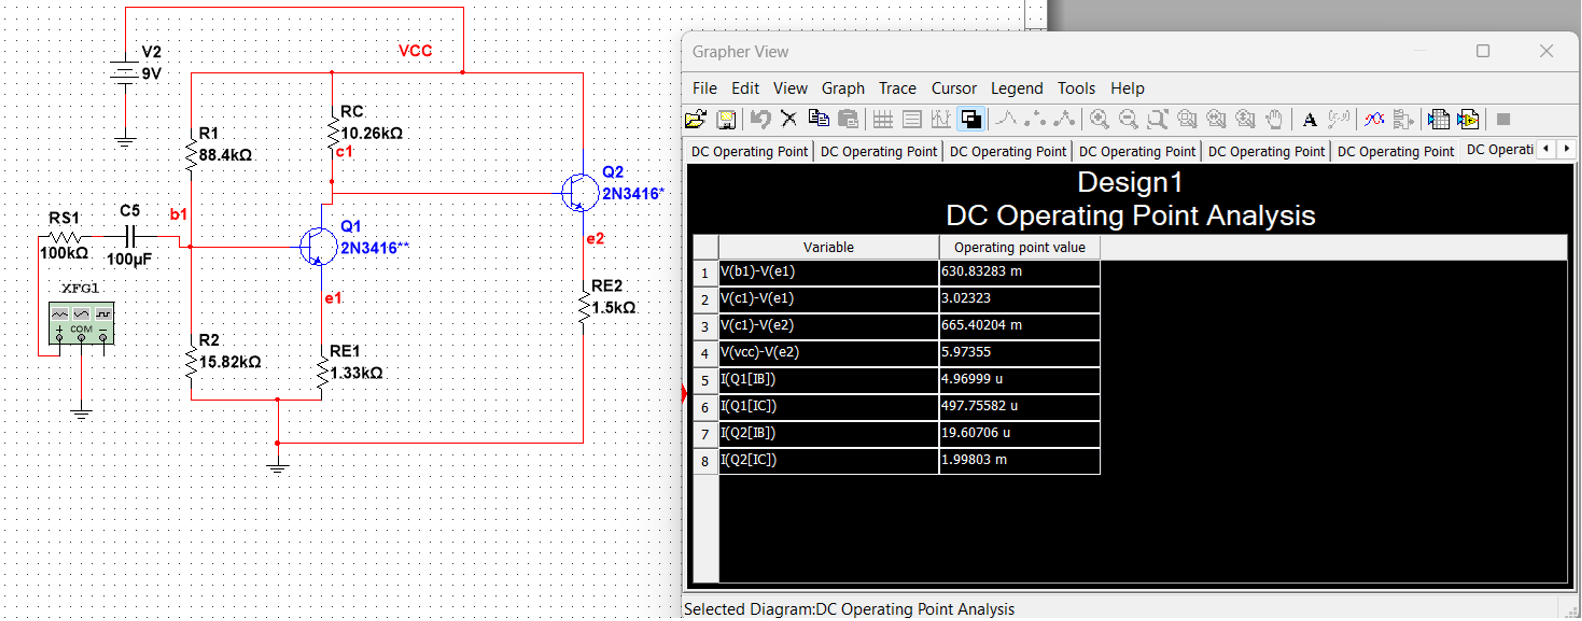
\includegraphics[width=.8\linewidth]{./my-chapters/my-images/Question9/a_diem_q.png}
		\caption{DC Point.}
	\end{figure}
	
\answer{b}{Đặt nguồn $v_{s} = V_{m}\sin\left(\omega t\right)$ có nội trở $R_{S} = 100\,\textsf{k}\Omega$ vào mạch. Ngõ ra nối với tải $R_{L}=1\,\textsf{k}\Omega$. Tìm $A_{vo}$, $A_{v}$, $G_{v}$, $R_{i}$, $R_{o}$ của mạch.}

Từ kết quả câu a ta có mạch như sau,

\begin{figure}[H]
	\centering
	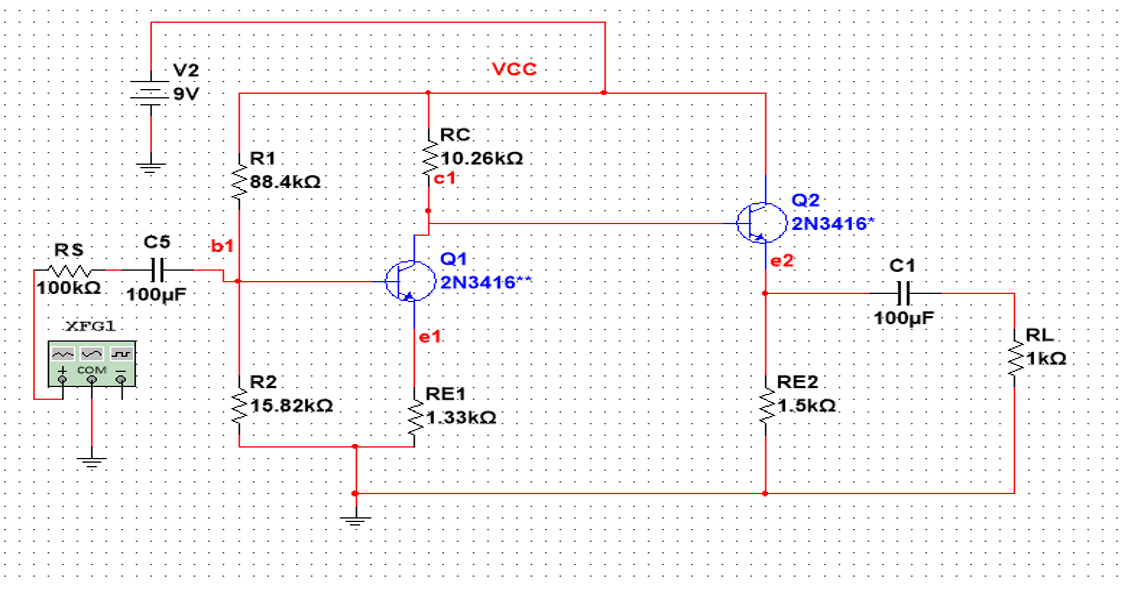
\includegraphics[width=.8\linewidth]{./my-chapters/my-images/Question9/b_debai.png}
\end{figure}

Ta chia thành 2 tầng như sau:
\begin{figure}[H]
	\centering
	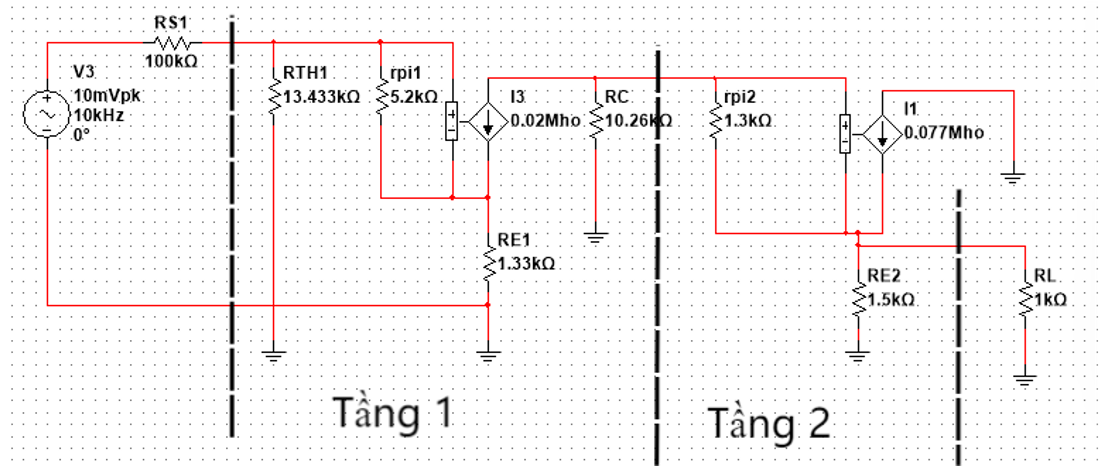
\includegraphics[width=.8\linewidth]{./my-chapters/my-images/Question9/b_sotang.png}
\end{figure}

\begin{itemize}[label=+, leftmargin=2cm]
	\item \( r_{\pi1} = \dfrac{V_T}{I_{B1}} = \dfrac{V_T  \beta}{I_{CQ1}} = \dfrac{26  100}{0.5} = 5.2\,k\Omega \)
	\item \( r_{\pi2} = \dfrac{V_T}{I_{B2}} = \dfrac{V_T  \beta}{I_{CQ2}} = \dfrac{26  100}{2} = 1.3\,k\Omega \)
	\item \( g_{m1} = \dfrac{I_{CQ1}}{V_T} = \dfrac{0.5}{26} = 0.02\,(\text{S}) \)
	\item \( g_{m2} = \dfrac{I_{CQ2}}{V_T} = \dfrac{2}{26} = 0.077\,(\text{S}) \)
\end{itemize}

\begin{itemize}[label=-]
	\item Tầng 1
		
		\begin{itemize}[label=+, leftmargin=2cm]
			\item \( R_{in1} = R_{TH1} // (r_{\pi1} + (\beta + 1) R_{E1}) 
			= 13.433\,k // (5.2\,k + 101 \times 1.33\,k) 
			= 12.25\,k\Omega \)
			
			\item \( R_{out1} = R_{C1} = 10.26\,k\Omega \)
			
			\item \( A_{V1} = 
			\dfrac{-\beta  R_C}{r_{\pi1} + (\beta + 1) R_{E1}} 
			= \dfrac{-100  10.26\,k}{5.2\,k + 101  1.33\,k} 
			= -7.35\,(\text{V/V}) \)
		\end{itemize}
		
	\item Tầng 2
	
		\begin{itemize}[label=+, leftmargin=2cm]
			\item \( R_{in2} = r_{\pi2} + (\beta + 1) R_{E2} 
			= 1.3\,k + 101 \times 1.5\,k 
			= 152.8\,k\Omega \)
			
			\item \( R_{out2} = R_{E2} // \dfrac{r_{\pi2}}{(\beta + 1)} 
			= 1.5\,k // \dfrac{1.3\,k}{101} 
			= 0.0137\,k\Omega \)
			
			\item \( A_{V2} = 
			\dfrac{R_{E2}}{R_{E2} + \dfrac{r_{\pi2}}{(\beta + 1)}} 
			= \dfrac{1.5\,k}{1.5\,k + \dfrac{1.3\,k}{101}} 
			= 0.99\,(\text{V/V}) \)
		\end{itemize}
	\item Toàn bộ tầng
	
		\begin{itemize}[label=+, leftmargin=2cm]
			\item \finalresult{R_{in} = R_{in1} = 12.25\,k\Omega}
			
			\item \finalresult{R_{out} = R_{out2} = 0.013\,k\Omega }
			
			\item \( A_{vo} = A_{v1} A_{v2} 
			\dfrac{R_{in2}}{R_{out1} + R_{in2}} 
			= -6.82\,(\text{V/V}) \)
			
			$\Rightarrow$ \finalresult{A_{vo} = -6.82\,(\text{V/V})}
			\item \( A_V = A_{V0} 
			\dfrac{R_L}{R_{out} + R_L} 
			= -6.73\,(\text{V/V}) \)
			
			$\Rightarrow$ \finalresult{A_{v} = -6.73\,(\text{V/V})}
			\item \( G_V = A_V 
			\dfrac{R_{in}}{R_{in} + R_S} 
			= -0.73\,(\text{V/V}) \)
			
			$\Rightarrow$ \finalresult{G_{v} = -0.73\,(\text{V/V})}
		\end{itemize}
	\item Kiểm tra kết quả
	
	\begin{figure}[H]
		\centering
		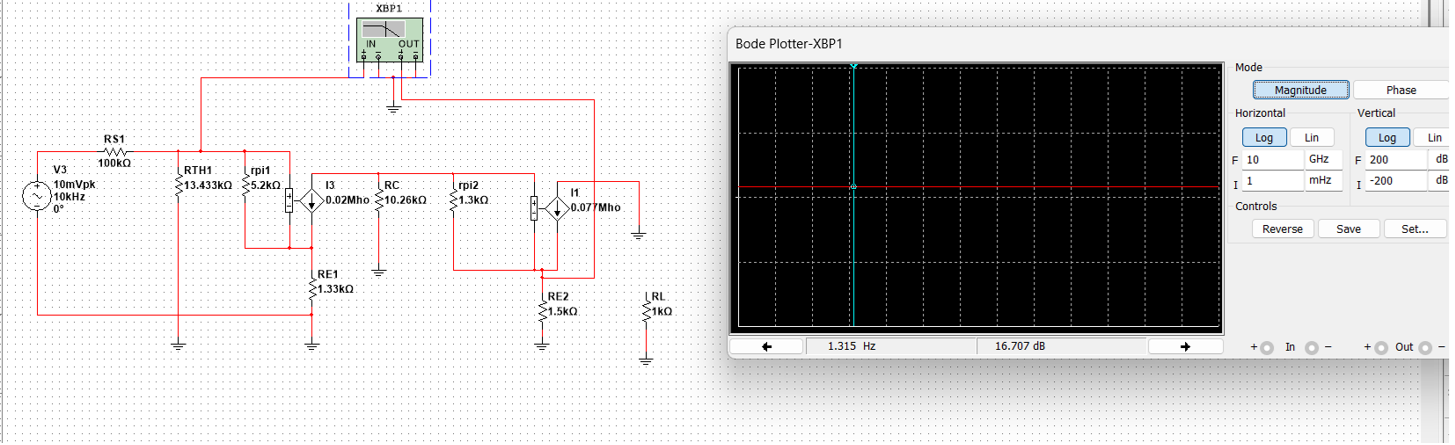
\includegraphics[width=.8\linewidth]{./my-chapters/my-images/Question9/b_avo.png}
		\caption{Đo \(|A_{V0}|\) = \(16.707\,\text{dB} = 6.84\,\text{V/V}\) (mô hình tương đương)}
	\end{figure}
	
	\begin{figure}[H]
		\centering
		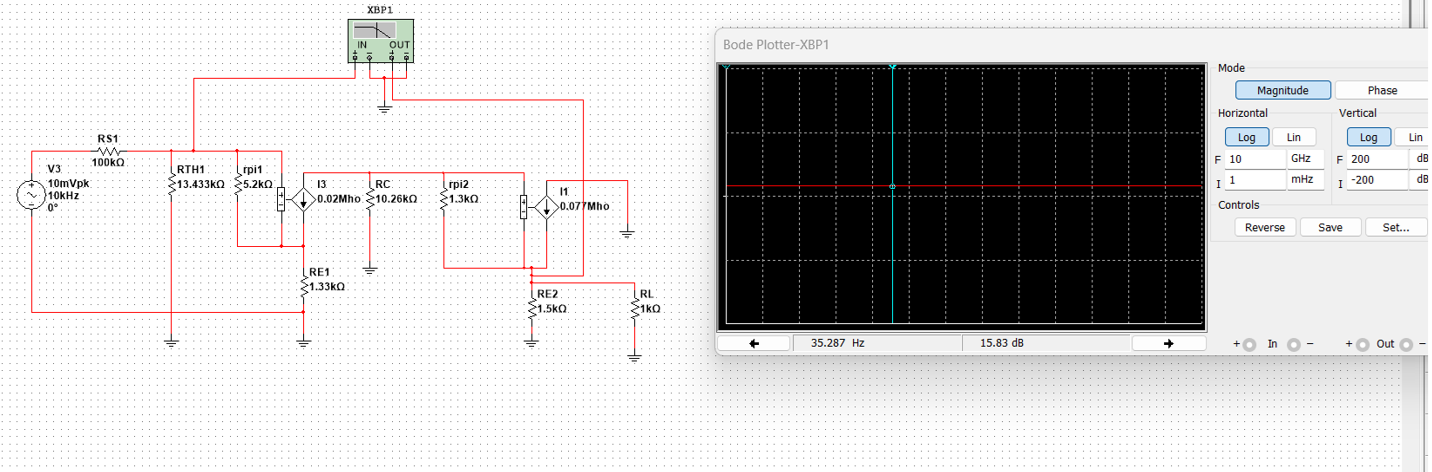
\includegraphics[width=.8\linewidth]{./my-chapters/my-images/Question9/b_av.png}
		\caption{Đo \(|A_{V}|\) = \(15.83\,\text{dB} = 6.187\,\text{V/V}\) (mô hình tương đương)}
	\end{figure}
	
	\begin{figure}[H]
		\centering
		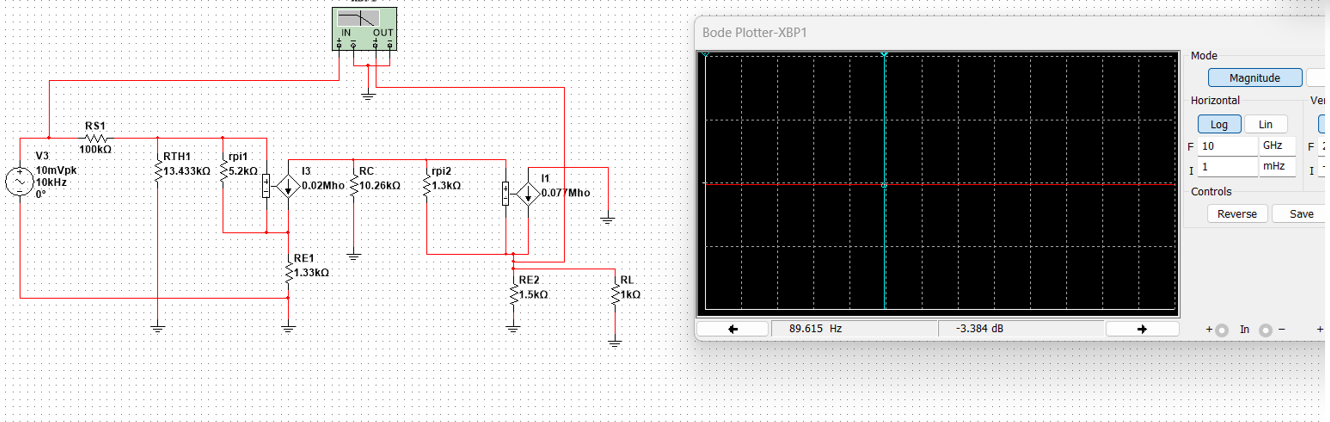
\includegraphics[width=.8\linewidth]{./my-chapters/my-images/Question9/b_gv.png}
		\caption{Đo \(|G_{V}|\) = \(-3.384\,\text{dB} = 0.677\,\text{V/V}\) (mô hình tương đương)}
	\end{figure}
	
	\begin{figure}[H]
		\centering
		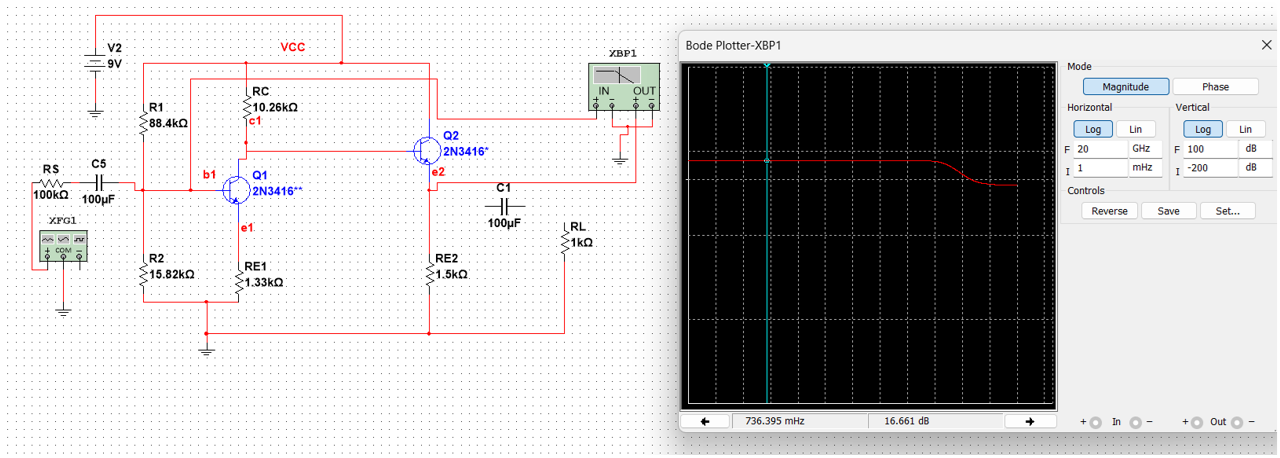
\includegraphics[width=.8\linewidth]{./my-chapters/my-images/Question9/b_avo_toan.png}
		\caption{Đo \(|A_{V0}|\) = \(16.661\,\text{dB} = 6.77\,\text{V/V}\) (toàn mạch)}
	\end{figure}
	
	\begin{figure}[H]
		\centering
		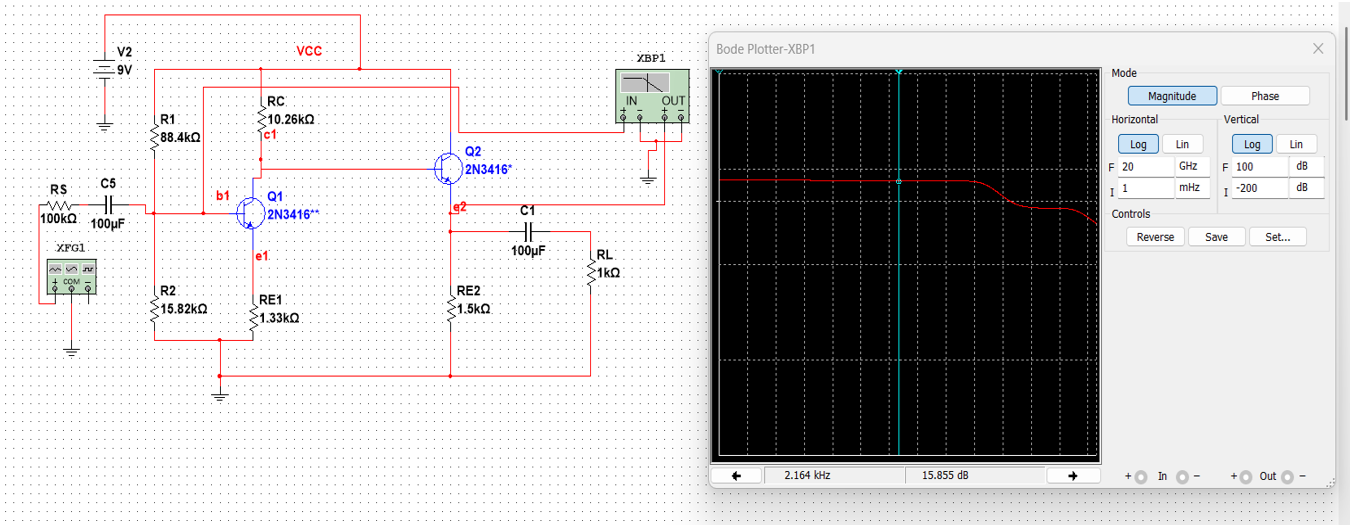
\includegraphics[width=.8\linewidth]{./my-chapters/my-images/Question9/b_av_toan.png}
		\caption{Đo \(|A_{V}|\) = \(15.855\,\text{dB} = 6.20\,\text{V/V}\) (toàn mạch)}
	\end{figure}
	
	\begin{figure}[H]
		\centering
		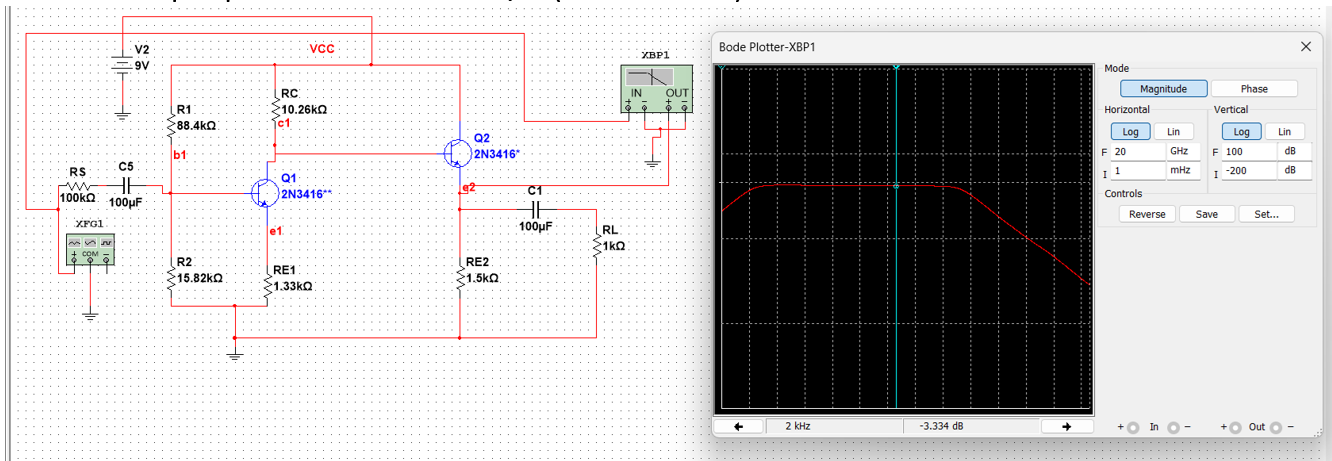
\includegraphics[width=.8\linewidth]{./my-chapters/my-images/Question9/b_gv_toan.png}
		\caption{Đo \(|G_{V}|\) = \(-3.34\,\text{dB} = 0.68\,\text{V/V}\) (toàn mạch)}
	\end{figure}
\end{itemize}

\answer{c}{Tìm biên độ lớn nhất của $V_{m}$ để để $v_{s}$ là tín hiệu nhỏ ở cả hai tầng.}

\begin{figure}[H]
	\centering
	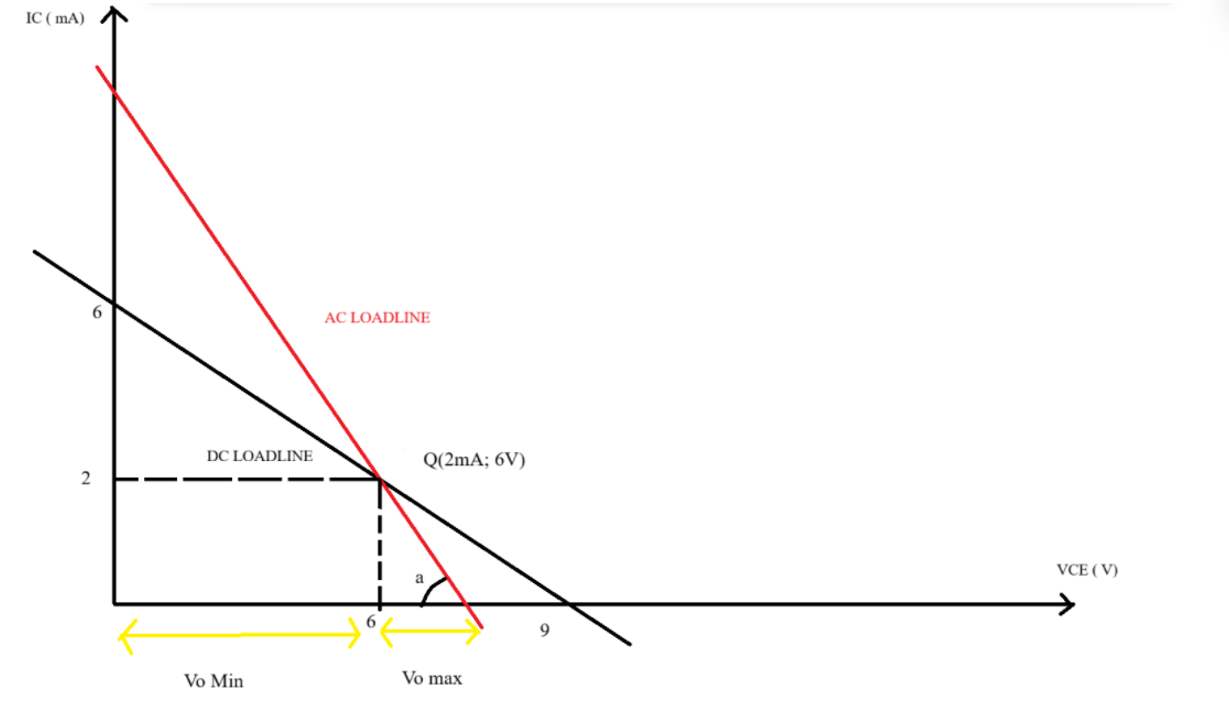
\includegraphics[width=.8\linewidth]{./my-chapters/my-images/Question9/c_dcloadline.png}
\end{figure}

\[
\tan(\alpha) = \frac{1}{R_L // R_{E2}} 
= \frac{1}{0.6\,k}
\;\Rightarrow\;
V_{o,\text{max}} = \frac{I_{CQ2}}{\tan(\alpha)} 
= 1.2\,\text{V}
\]

\[
V_{\text{sig,max}} = 
\frac{V_{o,\text{max}}}{G_V(f = 2\,\text{kHz})} 
= \frac{1.2}{0.68} 
= 1.76\,\text{V}
\]

$\Rightarrow$ \finalresult{V_{\text{sig,max}} = 1.76\,\text{V}}

\begin{figure}[H]
	\centering
	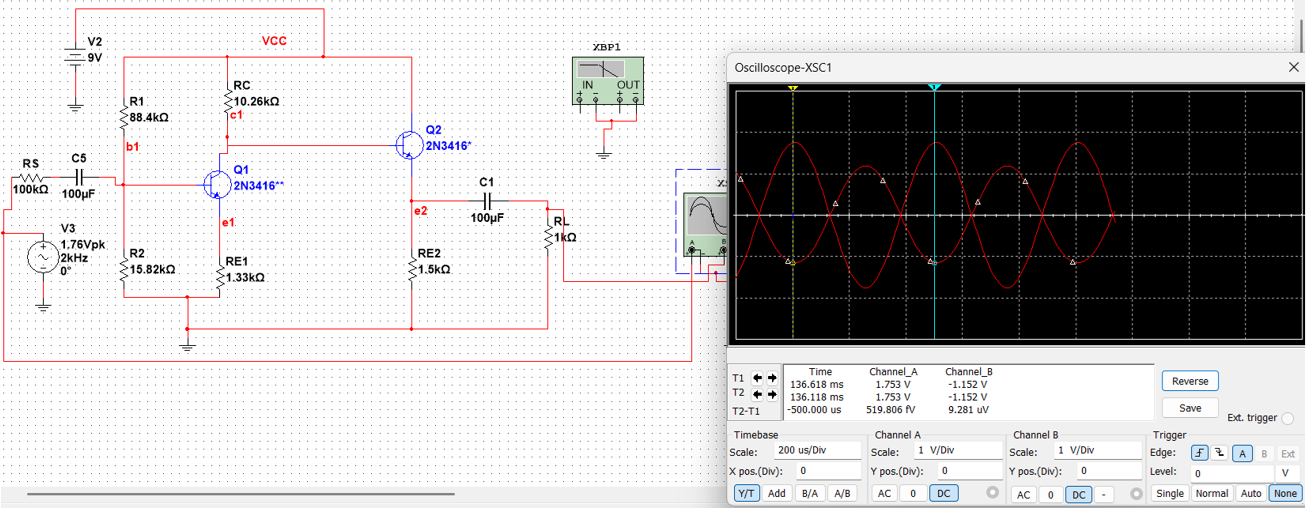
\includegraphics[width=.8\linewidth]{./my-chapters/my-images/Question9/c_1.png}
	\caption{\(V_{p,\text{sig}} = 1.76\,\text{V};\ 
		V_{pL} = -1.152\,\text{V};\ 
		G_V = -0.654\,(\text{V/V})\)}
\end{figure}

\begin{figure}[H]
	\centering
	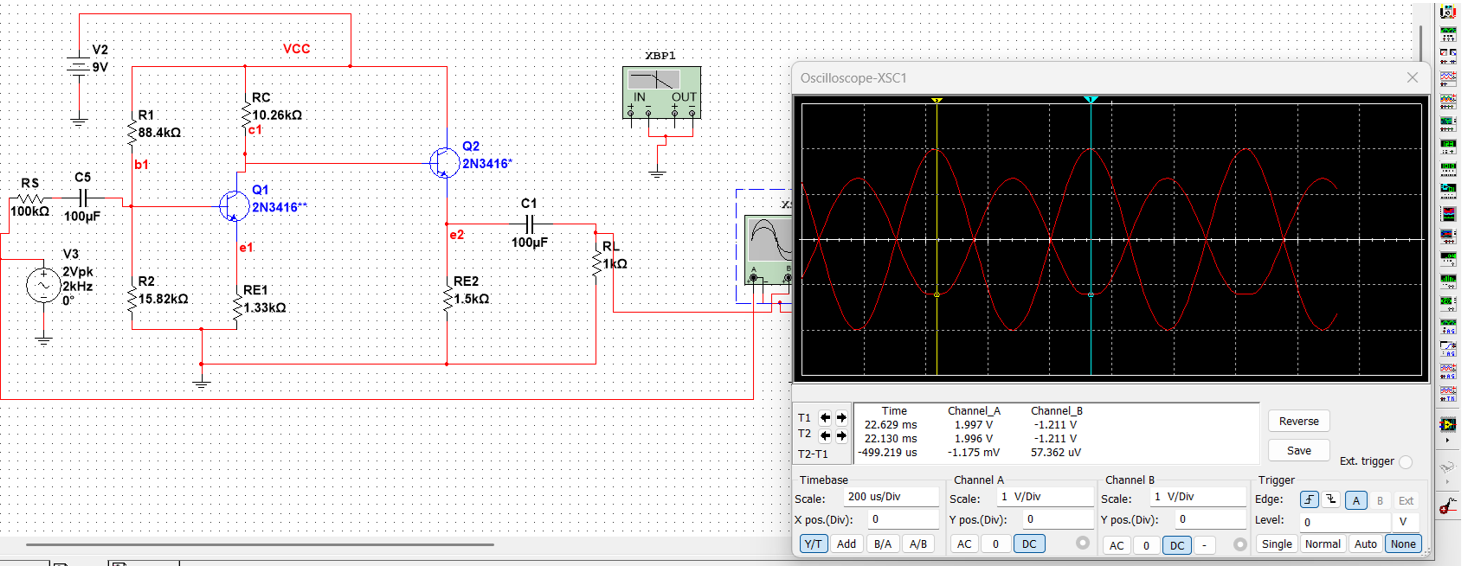
\includegraphics[width=.8\linewidth]{./my-chapters/my-images/Question9/c_2.png}
	\caption{\(V_{p,\text{sig}} = 2\,\text{V};\ 
		V_{pL} = -1.211\,\text{V};\ 
		G_V = -0.6055\,(\text{V/V})\) 
		(ngõ ra đã bị xén dưới)}
\end{figure}

\answer{d}{Thiết kế mắc thêm tụ $C$ để cải thiện độ lợi của mạch. Tính lại $G_{v}$, $R_{i}$, $R_{o}$ của mạch.}

\begin{figure}[H]
	\centering
	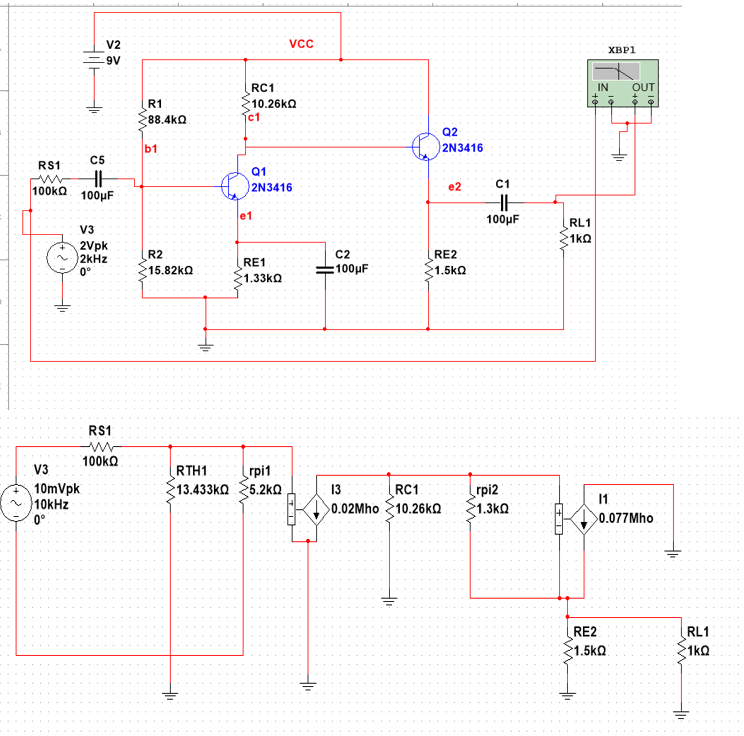
\includegraphics[width=.8\linewidth]{./my-chapters/my-images/Question9/d_de.png}
	\caption{Mắc các tụ $C$ vào mạch.}
\end{figure}

\begin{itemize}[label=+, leftmargin=2cm]
	\item \( r_{\pi1} = \dfrac{V_T}{I_{B1}} = \dfrac{V_T \, \beta}{I_{CQ1}} 
	= \dfrac{26 \times 100}{0.5} = 5.2\,k\Omega \)
	
	\item \( r_{\pi2} = \dfrac{V_T}{I_{B2}} = \dfrac{V_T \, \beta}{I_{CQ2}} 
	= \dfrac{26 \times 100}{2} = 1.3\,k\Omega \)
	
	\item \( g_{m1} = \dfrac{I_{CQ1}}{V_T} = \dfrac{0.5}{26} = 0.02\,(\text{S}) \)
	
	\item \( g_{m2} = \dfrac{I_{CQ2}}{V_T} = \dfrac{2}{26} = 0.077\,(\text{S}) \)
\end{itemize}

\begin{itemize}[label=-]
	\item Tầng 1
	\begin{itemize}[label=+, leftmargin=2cm]
		\item \( R_{in1} = R_{TH1} // r_{\pi1} 
		= 13.433\,k // 5.2\,k 
		= 3.75\,k\Omega \)
		
		\item \( R_{out1} = R_C = 10.26\,k\Omega \)
		
		\item \( A_{V1} = -g_{m1} R_C 
		= -0.02 \times 10.26\,k 
		= -205.2\,(\text{V/V}) \)
	\end{itemize}
	
	\item Tầng 2
	\begin{itemize}[label=+, leftmargin=2cm]
		\item \( R_{in2} = r_{\pi2} + (\beta + 1) R_{E2} 
		= 1.3\,k + 101 \times 1.5\,k 
		= 152.8\,k\Omega \)
		
		\item \( R_{out2} = R_{E2} // \dfrac{r_{\pi2}}{(\beta + 1)} 
		= 1.5\,k // \dfrac{1.3\,k}{101} 
		= 0.0137\,k\Omega \)
		
		\item \( A_{V2} = 
		\dfrac{R_{E2}}{R_{E2} + \dfrac{r_{\pi2}}{(\beta + 1)}} 
		= \dfrac{1.5\,k}{1.5\,k + \dfrac{1.3\,k}{101}} 
		= 0.99\,(\text{V/V}) \)
	\end{itemize}
	
	\item Toàn bộ tầng
	\begin{itemize}[label=+, leftmargin=2cm]
		\item \finalresult{R_{in} = R_{in1} = 3.75\,k\Omega}
		
		\item \finalresult{R_{out} = R_{out2} = 0.013\,k\Omega}
		
		\item \( A_{V0} = A_{V1} A_{V2} 
		\dfrac{R_{in2}}{R_{out1} + R_{in2}} 
		= -190.36\,(\text{V/V}) \)
		
		$\Rightarrow$ \finalresult{A_{V0} = -190.36\,(\text{V/V})}
		
		\item \( A_V = A_{V0} 
		\dfrac{R_L}{R_{out} + R_L} 
		= -187.92\,(\text{V/V}) \)
		
		$\Rightarrow$ \finalresult{A_V = -187.92\,(\text{V/V})}
		
		\item \( G_V = A_V 
		\dfrac{R_{in}}{R_{in} + R_S} 
		= -6.79\,(\text{V/V}) \)
		
		$\Rightarrow$ \finalresult{G_V = -6.79\,(\text{V/V})}
	\end{itemize}
	\item Kiểm tra kết quả
	
	\begin{figure}[H]
		\centering
		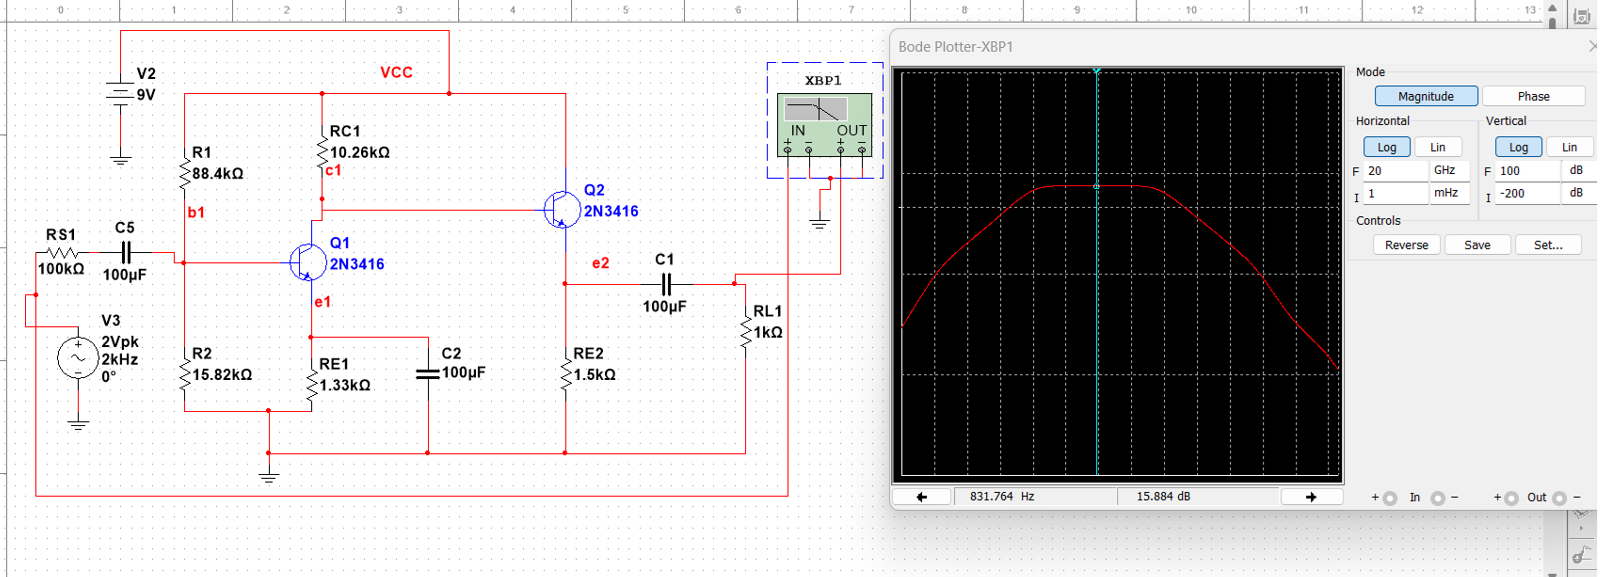
\includegraphics[width=.8\linewidth]{./my-chapters/my-images/Question9/d_result.png}
		\caption{Đo $|G_{v}| = 15.884db = 6.225 \,\textsf{(V/V)}$}
	\end{figure}
\end{itemize}
